\documentclass[12pt,letterpaper]{article}
\usepackage[utf8]{vietnam}
\usepackage{fullpage}
\usepackage[top=2cm, bottom=4.5cm, left=2.5cm, right=2.5cm]{geometry}
\usepackage{amsmath,amsthm,amsfonts,amssymb,amscd}
\usepackage{lastpage}
\usepackage{enumerate}
\usepackage{fancyhdr}
\usepackage{mathrsfs}
\usepackage{xcolor}
\usepackage{graphicx}
\usepackage{listings}
\usepackage{hyperref}

\hypersetup{%
  colorlinks=true,
  linkcolor=blue,
  linkbordercolor={0 0 1}
}

\renewcommand\lstlistingname{Algorithm}
\renewcommand\lstlistlistingname{Algorithms}
\def\lstlistingautorefname{Alg.}

\lstdefinestyle{Python}{
    language        = Python,
    frame           = lines, 
    basicstyle      = \footnotesize,
    keywordstyle    = \color{blue},
    stringstyle     = \color{green},
    commentstyle    = \color{red}\ttfamily
}

\setlength{\parindent}{0.0in}
\setlength{\parskip}{0.05in}

% Edit these as appropriate
\newcommand\course{Massp2019}
\newcommand\hwnumber{Logistic and Softmax Regression}                  % <-- homework number
\newcommand\NetIDa{Nguyen Quang Huy}           % <-- NetID of person #1

\pagestyle{fancyplain}
\headheight 35pt
\lhead{\NetIDa}
%\lhead{\NetIDa\\\NetIDb}                 % <-- Comment this line out for problem sets (make sure you are person #1)
\chead{\textbf{\hwnumber}}
\rhead{\course \\ \today}
\lfoot{}
\cfoot{}
\rfoot{\small\thepage}
\headsep 1.5em

\begin{document}
\section*{Logistic Regression là gì}
Logistic Regression dùng để dự đoán xác suất, thường được ứng dụng trong các bài toán classification

Logistic Regression được tính bằng công thức:
$$
    y = \theta(w^T*x)
$$
trong đó $\theta$ là 1 hàm logistic function

Đầu ra của logistic Regression là giá trị trong khoảng [0,1] có ý nghĩa đưa ra xác suất

\section*{Softmax Regression là gì}
Trong thực tế, bài toán classìication thường có rất nhiều class. Khi đó, thuật toán Logistic Regression có hạn chế khi kết quả chỉ có thể phân chia làm 2 class "đúng" và "sai". Softmax Regression có thể hiểu như một mở rộng của Logistic Regression khi cho ra kết quả là 1 vector dự đoán xác suất của mỗi class của dữ liệu.

Softmax Regression được tính bằng công thức:
$$
    a_i = \frac{\theta(z_i)}{\sum_{j = 1}^{C}{\theta(z_j)}} , \forall i = 1,2,...,C 
$$
Tính chất của Softmax Regression:
\begin{enumerate}
    \item $ a_i $ là giá trị trong khoảng [0,1] $\forall i = 1,2,...,C $
    \item $\sum_{i=1}^C{a_i} = 1$
\end{enumerate}
\section*{Nhận xét}
Cả 2 thuật toán Logistic Regression và Softmax Regression đều tính xác suất và được ứng dụng trong bài toán classification
\\ 
2 thuật toán đều giải quyết vấn đề thuộc khoảng từ $Z_g$ đến $Z_x$ trong sơ đồ: 
\begin{figure}
    \centering
    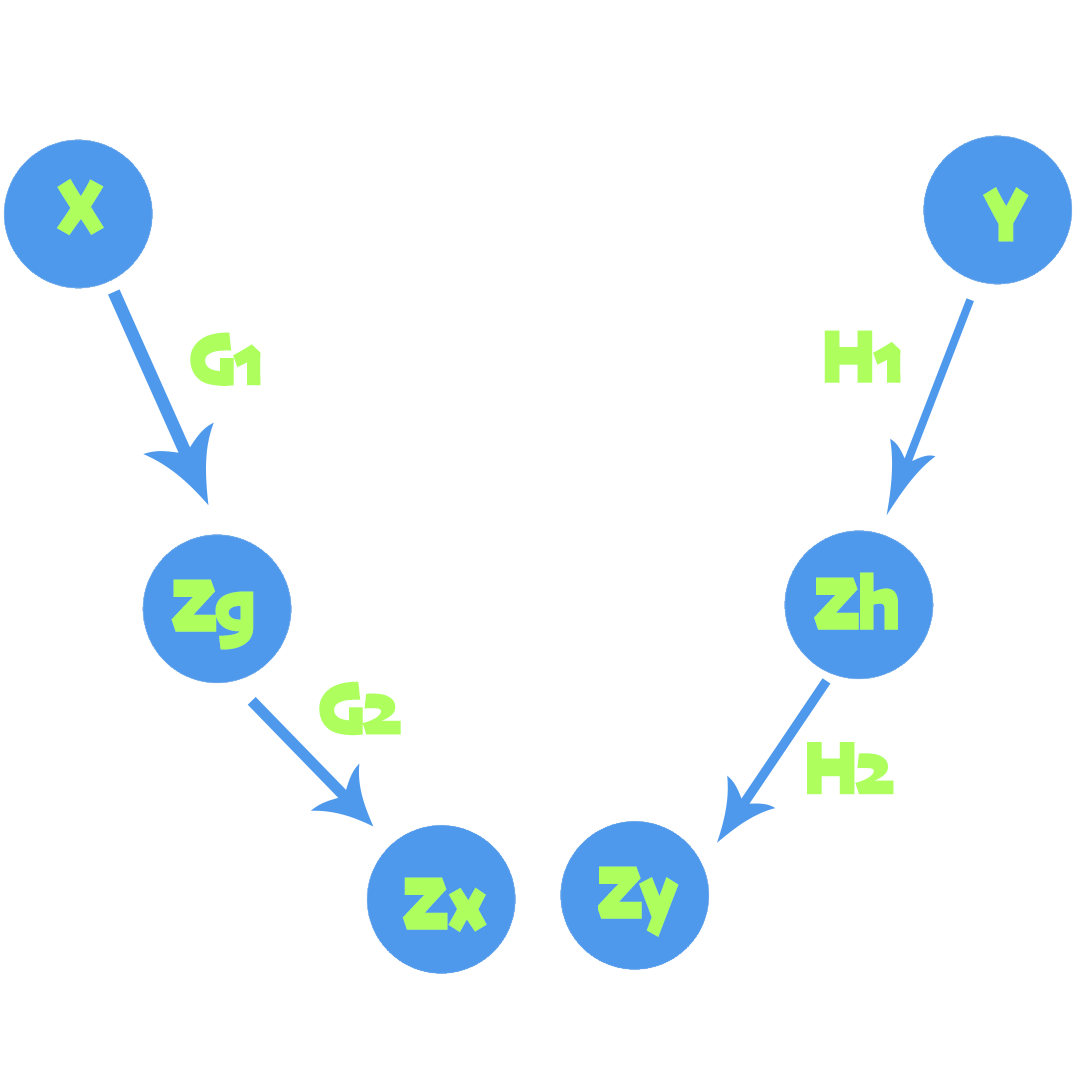
\includegraphics[width=1 \linewidth]{unifiedframework.png}
\end{figure}

\end{document}